\section{原子结构的玻尔理论}

\begin{quotation}
``当电子从一个定态过渡到另一个定态时,它怎么决定将以什么频率来振动呢?''\qquad 卢瑟福
\end{quotation}

\subsection{原子光谱}

\index{Spectrum: 光谱}

光谱是光的频率和强度分布的关系图, 是研究原子(和分子)结构的重要途径。
如果我们将充有某种原子蒸汽的``真空管''通电, 使之发光,
并测量发出光的光谱,
所测得的便是该元素(该原子)的光谱,即发射光谱(emission spectrum),
谱线是明线。另外一种光谱是吸收光谱(absorption spectrum),
谱线是暗线(低温原子气吸收波长连续分布光源中特定波长光形成)。
同一元素的发射谱线与吸收谱线一一对应。

实验发现相同元素原子谱线相同, 不同元素原子的谱线都不相同,
这些谱线成为辨认不同原子的``指纹''。 利用测量原子光谱的方法,
科学家们发现了很多新元素, 如:He(1862年), Cs(1860年), Rb(1861年)等。

一个关于原子的成功理论必须能解释原子光谱。

\begin{figure}[h]
\begin{center}
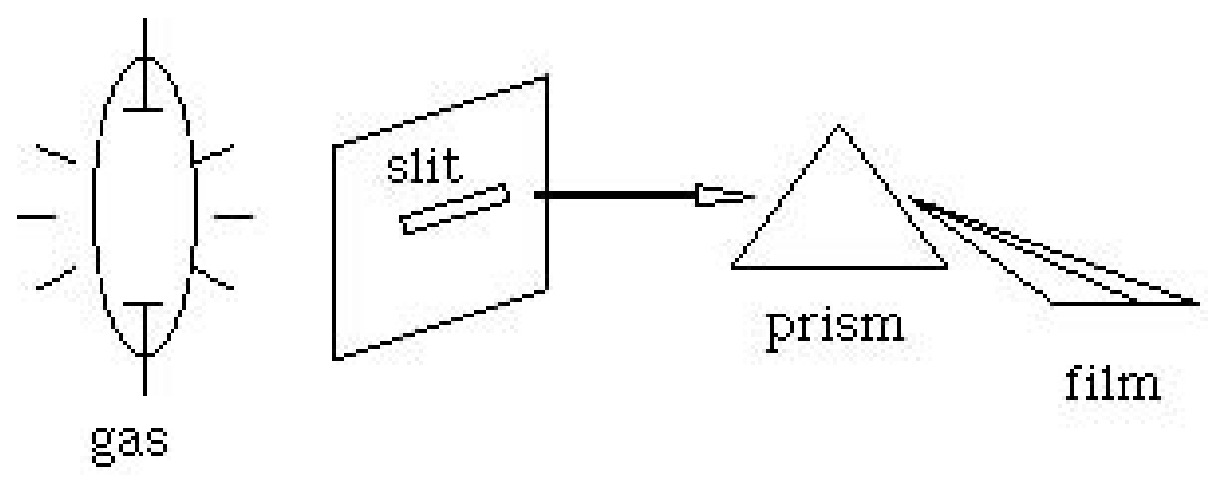
\includegraphics[clip,width=8cm]{BohrModel/4-1.ps}
\caption{原子光谱示意}
\end{center}
\end{figure}

19世纪末, 关于光谱学的实验研究取得了极大进展,
积累了大量实验数据需要整理, 以便从中找出规律, 作出理论解释。
这种情况颇类似于16世纪时第谷积累了大量关于行星运行的数据,
直接导致开普勒在此基础上提出开普勒定律以及后来牛顿建立经典力学理论体系。
目前分子生物学领域测量了各种基因、蛋白质的结构, 并获得大量数据,
但隐藏在这些数据背后的规律还有待我们去发现, 这些规律的发现,
将很可能导致新的科学革命。就象光谱学后来的发展直接导致了玻尔理论及量子力学一样。

\begin{figure}[h]
\begin{center}
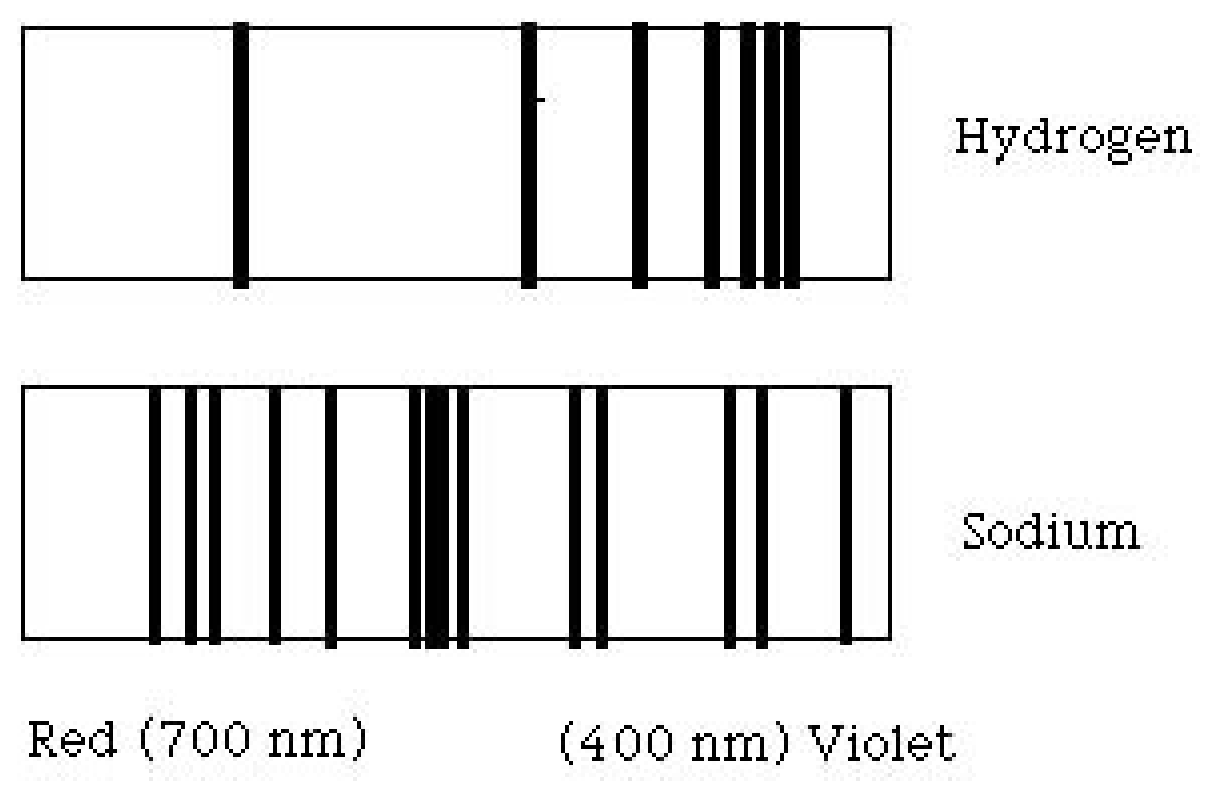
\includegraphics[clip,width=9cm]{BohrModel/4-2.ps}
\caption{氢光谱与钠光谱}
\end{center}
\end{figure}

\subsubsection{氢原子光谱经验规律}

1855年,瑞士中学教师巴尔末(Balmer)发现了关于氢原子光谱的经验公式:

\begin{equation}\label{Balmer's formula}
    \tilde \nu  = \frac{1}{\lambda } = \frac{4}{B}\left( {\frac{1}{{2^2 }} - \frac{1}{{n^2 }}} \right),n = 3,4,5...
\end{equation}

\index{Balmer's formula: 巴尔末公式}

其中:$B=364.56nm$, 这个公式被称为:巴尔末公式(Balmer's formula),
它所描述的这组谱线被称为巴尔末系(Balmer series)。

\index{Balmer series: 巴尔末系}

1889年, 里德堡(Rydberg)提出一个更普遍的方程:

\begin{equation}\label{Rydberg's formula}
    \tilde \nu  = \frac{1}{\lambda } = R_H \left( {\frac{1}{{n^2 }} - \frac{1}{{n'^2 }}} \right) = T(n) - T(n')
\end{equation}

这里:

\begin{equation}
R_H  = \frac{4}{B} = 1.097 \times 10^7 m^{ - 1},
\end{equation}

称为里德堡常数。$T(n)$称为光谱项,$n=1,2,3, ...$,$n' = n + 1,n + 2,n + 3...$

$n=1$时, 赖曼系;$n=2$时, 巴尔末系;$n=3$时, 帕刑系;$n=4$时,
布喇开系;$n=5$时, 普丰特系。

\subsubsection{经典理论的困难}

卢瑟福模型是迈向正确原子模型的关键一步,
但我们使用经典物理学处理卢瑟福模型, 必然得到如下结论:

\index{Rutherford model: 卢瑟福模型}

\begin{enumerate}
    \item 任何作加速运动的带电粒子都要辐射电磁波(即发光),发射电磁波,会使电子能量降低,导致电子轨道不断变小,
并最终落到原子核上,使原子``消失'';
    \item 由于电子能量可以连续变化,所发射电磁波能量也是连续的,原子光谱应是连续的。
由经验和原子半衰期数据知道,原子很稳定,而且原子光谱是线状的,并非连续的。
\end{enumerate}


\subsection{玻尔模型}

\begin{figure}[h]
\begin{center}
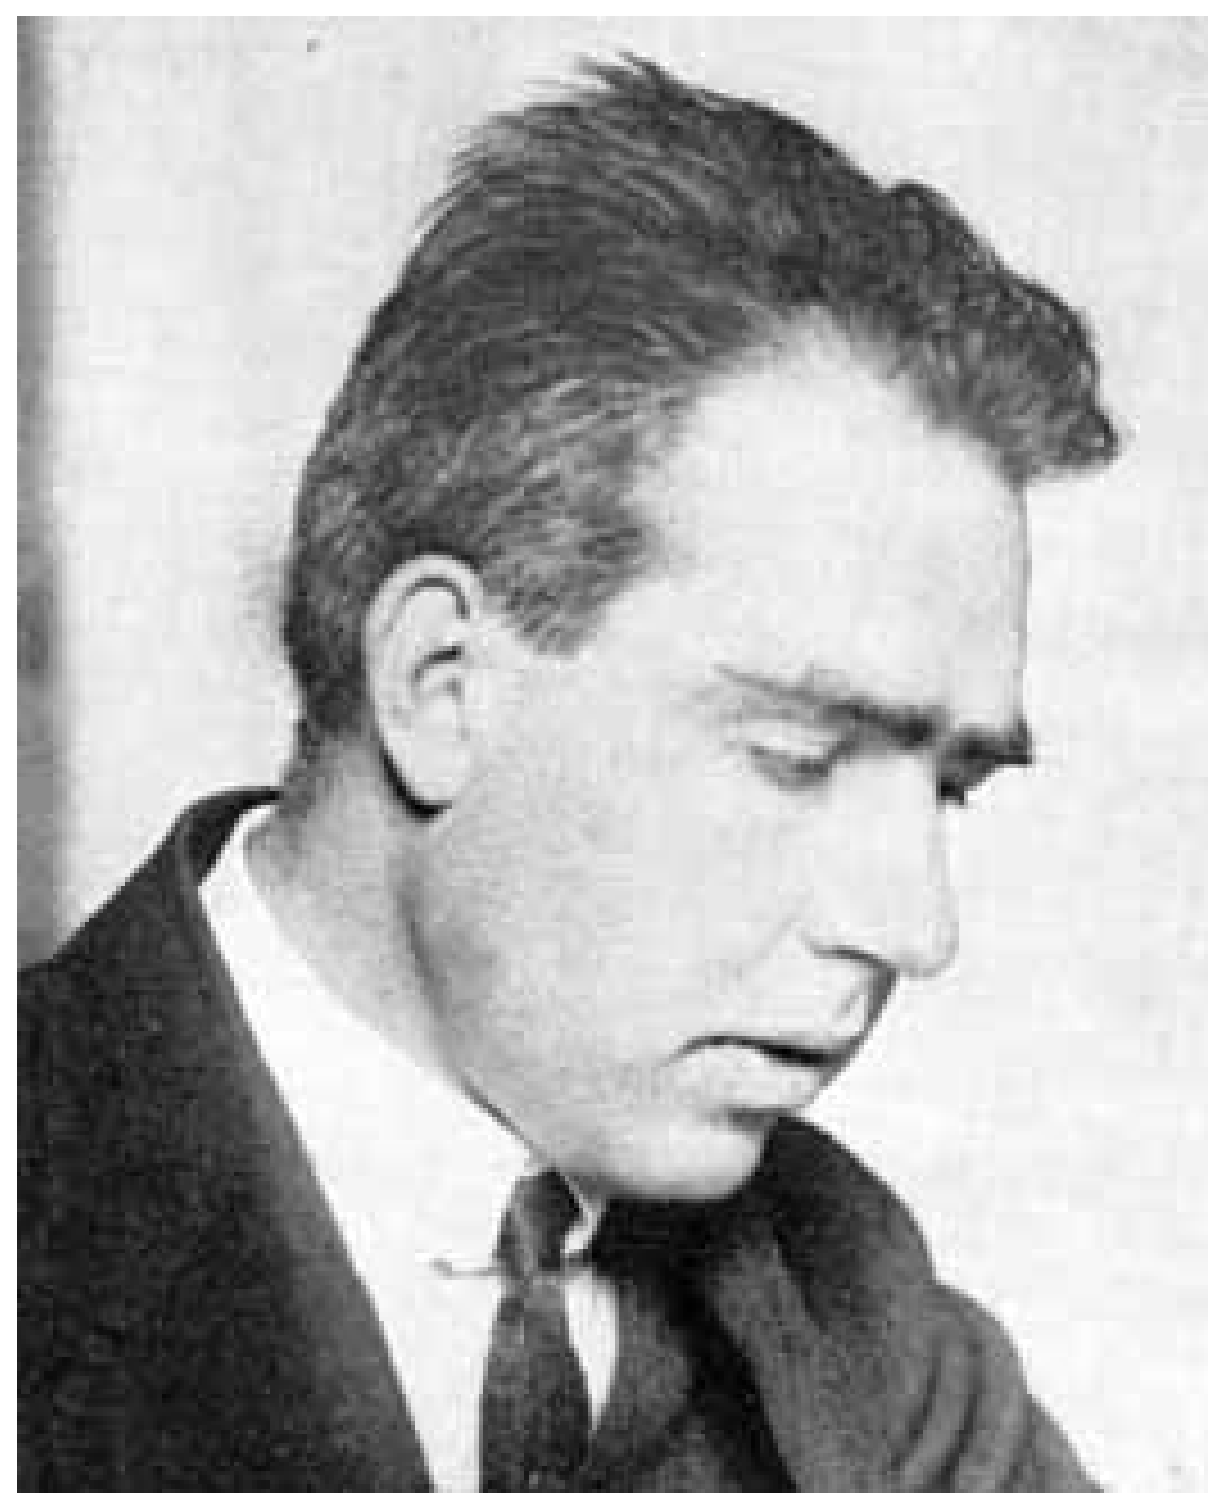
\includegraphics[clip,width=4cm]{BohrModel/bohr.ps}
\caption{玻尔}
\end{center}
\end{figure}

\index{Bohr model: 玻尔模型}

1913年, 玻尔(N. Bohr)正在卢瑟福的实验室工作,
他基于卢瑟福的有核模型(即行星模型, planetary model),
普朗克的量子(quanta)和爱因斯坦的光子(photon)概念解释了氢原子光谱。玻尔的理论基于三个武断的假设,
这三个假设与已有理论——经典力学,经典电磁学——是矛盾的,
而且玻尔也没有真正建立一个全新的理论,
严格意义上的量子力学要在后来才被建立。但玻尔的半截子理论很好地描述了氢原子光谱,
说明他引入的``定态(stationary
state)''等概念对建立量子力学是非常关键的,
这个理论在科学史上被称作旧量子论(Old quantum theory)。

\index{Stationary state: 定态}

\index{Old quantum theory: 旧量子论}

\begin{description}
    \item[定态假设] 原子中存在定态,定态能量取离散值$E_1 ,E_2 ,E_3 ...$。原子在定态时不辐射也不吸收电磁波,玻尔明确指出在氢原子中的定态就是一系列电子围绕原子核的正圆周轨道运动。
    \item[频率条件] 电子在不同定态$E_1 ,E_2 $间可发生跃迁,以发射或吸收特定频率$\nu$光子的形式进行,满足能量守恒,

\begin{equation}
h \nu = E_2 - E_1
\end{equation}

$h$为普郎克常数。频率$\nu$满足:
    
\begin{equation}
\nu  = \frac{{E_2  - E_1 }}{h}.
\end{equation}
    
    \item[角动量量子化] 那么哪些圆周运动才是允许的定态呢,玻尔通过轨道角动量(orbital angular momentum)量子化给出:
    
\begin{equation}
L = n\hbar
\end{equation}

这里:

\begin{equation}
\hbar  = h/2\pi = 1.054572 \times 10^{-34} Js = 6.582119 \times 10^{-16} eV s  
\end{equation}

叫作约化普朗克常数(reduced Planck constant)。

\end{description}

由以上假设不难看出, 玻尔是在经典物理的框架内提出``定态''概念的,
所以玻尔的理论在逻辑上是不自恰的,比如为什么电子可以做圆周运动却不向外辐射电磁波等。要避免这类困难,
必须把``定态''概念重新建立在全新的量子力学基础上。但我们先不管这些,
看看在以上假设下能算出来些什么。

氢原子是由一个电子和一个质子组成,由于$m_e  \ll m_p
$,按单体问题处理。运动方程:

\begin{equation}
F = m_e \frac{{v^2 }}{r} = \frac{1}{{4\pi \varepsilon _0 }}\frac{{e^2 }}{{r^2 }}
\end{equation}

总能量:

\begin{equation}
E = T + V = {\textstyle{1 \over 2}}m_e v^2  - \frac{{e^2 }}{{4\pi \varepsilon _0 r}} =  - \frac{{e^2 }}{{8\pi \varepsilon _0 r}}
\end{equation}

\index{Quantization of angular momentum: 角动量量子化}

利用角动量量子化条件:$L = n\hbar  = m_e vr$:

\begin{equation*}
F = \frac{{e^2 }}{{4\pi \varepsilon _0 r^2 }} = \frac{{(m_e vr)^2 }}{{m_e r^3 }} = \frac{{\left( {n\hbar } \right)^2 }}{{m_e r^3 }}
\end{equation*}

化简可得:

\begin{equation*}
\frac{{e^2 }}{{4\pi \varepsilon _0 }} = \frac{{n^2 \hbar ^2 }}{{m_e r}}
\end{equation*}

最后得到:

\begin{equation}
r_n  = \frac{{4\pi \varepsilon _0 n^2 \hbar ^2 }}{{m_e e^2 }}
\end{equation}

这意味着电子的半径只能取分立的值$r_n$,即量子化的了。这样,能量也将量子化:

\begin{equation}
E_n  =  - \frac{{m_e e^4 }}{{\left( {4\pi \varepsilon _0 } \right)^2  \cdot 2\hbar ^2 n^2 }} =  - \frac{{m_e c^2 }}{2}\left( {\frac{{e^2 }}{{4\pi \varepsilon _0 \hbar c}}} \right)^2  \cdot \frac{1}{{n^2 }}
\end{equation}

\index{Fine-structure constant: 精细结构常数}

定义精细结构常数(fine structure constant, $\alpha$):

\begin{equation}
\alpha = \frac{{e^2 }}{{4\pi \varepsilon _0 \hbar c}} \simeq
\frac{1}{{137}}
\end{equation}

所以:

\begin{equation}
\tilde \nu  = \frac{1}{\lambda } = \frac{\nu }{c} = \frac{1}{{2hc}}m_e \left( {\alpha c} \right)^2 \left( {\frac{1}{{n^2 }} - \frac{1}{{n'^2 }}} \right)
\end{equation}

即里德堡公式。里德堡常数为: 

\begin{equation}
R_H = \frac{1}{{2hc}}m_e \left( {\alpha c} \right)^2
\end{equation}

通过玻尔模型可引入几个重要物理量:

\begin{description}
    \item[第一玻尔半径] n=1时,氢原子半径:
    
\begin{equation}
a_0  = r_1  = \frac{{4\pi \varepsilon _0 \hbar ^2 }}{{m_e e^2 }} \simeq 0.053 nm
\end{equation}

这样电子轨道半径$r_n$可表示为极简单的形式:
    
\begin{equation}
r_n  = a_0 n^2
\end{equation}


    \item[氢原子电离能] 把氢原子电子从基态(n=1)移到无限远($n = \infty $)所需要的能量,
    
\begin{equation}
E_\infty   = \frac{{m_e }}{2}\left( {\alpha c} \right)^2  = 13.6eV
\end{equation}

    \item[玻尔第一速度] 在基态氢原子中电子作圆周运动时的速度:
    
\begin{equation}
v_1  = \frac{\hbar }{{m_e r_1 }} = \frac{\hbar }{{m_e }}\frac{{m_e e^2 }}{{4\pi \varepsilon _0 \hbar ^2 }} = \frac{{e^2 }}{{4\pi \varepsilon _0 \hbar }}\frac{c}{c} = \alpha c
\end{equation}

即电子在氢原子中运动速度为光速的1/137,所以不需考虑相对论效应。

\end{description}

\subsection{玻尔模型的实验验证}

\subsubsection{氢光谱和类氢光谱}

如考虑到原子核不是无穷大情形, $m_e $应由折合质量$\mu  = \frac{{m_e
M}}{{m_e  + M}}$代替, 修正后的里德堡常数应为:

\index{Reduced mass: 折合质量}

\begin{equation}\label{revised Rydberg}
    R_A  = \frac{1}{{2hc}}(\alpha c)^2 \frac{{m_e M}}{{m_e  + M}} = R \cdot \frac{1}{{1 + {\textstyle{{m_e } \over M}}}}
\end{equation}

修正后的里德堡常数与实验测得数据完全吻合。这样,就完全解释了氢光谱的实验数据\footnote{
氢原子里德堡常数的实验值及考虑折合质量修正后的理论值:$R_H =
109677.58 cm^{-1}$, 不考虑折合质量修正时:$R = 109737.315
cm^{-1}$;}。

类氢离子:原子核外只有一个电子的离子, 原子核带正电荷$Ze$
如:He+,Li2+,Be3+等.

对类氢离子, 由于$M \gg m$, 只需考虑电子的单体运动. 电子的总能量是:

\begin{equation*}
E = T+V = \frac{mv^2}{2}- \frac{Ze^2}{4\pi \epsilon_0 r}
\end{equation*}

假设电子作正圆运动, 向心力:

\begin{equation}\label{centripetal force}
\frac{mv^2}{r} = \frac{Ze^2}{4\pi \epsilon_0 r^2}
\end{equation}

考虑``角动量量子化'',

\begin{equation*}
mvr = n \hbar, n=1,2,3,...
\end{equation*}

由公式(\ref{centripetal force}), 可得到:

\begin{equation*}
\frac{n^2 \hbar^2}{mr}=\frac{Ze^2}{4\pi \epsilon_0 }
\end{equation*}

因此轨道半径是``量子化''的,

\begin{equation*}
r_n = \frac{1}{Z}  \frac{4\pi \epsilon_0 n^2 \hbar^2}{me^2}
\end{equation*}

代入到能量的表达式中:

\begin{equation*}
E = - \frac{mv^2}{2} = - \frac{Ze^2}{8 \pi \epsilon_0 r}
\end{equation*}

得到``能量量子化'',

\begin{equation*}
E_n = - Z^2 \frac{me^4}{32 \pi^2 \epsilon_0^2 n^2 \hbar^2}
\end{equation*}

电子速度:

\begin{equation*}
v_n = Z \frac{e^2}{4 \pi \epsilon_0 n \hbar}
\end{equation*}


考虑到精细结构常数:  $\alpha = \frac{e^2}{4\pi \epsilon_0 \hbar c}
$, $r_n$, $E_n$ 和 $v_n$可重新写为:

\begin{eqnarray*}
% \nonumber to remove numbering (before each equation)
  r_n &=& \frac{1}{Z} \cdot \frac{ \hbar}{m c \alpha} \cdot n^2 \\
  E_n &=& - Z^2 \cdot \frac{mc^2}{2} \alpha^2 \cdot \frac{1}{n^2} \\
  v_n &=& Z \cdot c \alpha \cdot \frac{1}{n}
\end{eqnarray*}


即:类氢原子($Z \ne 1$)与氢原子($Z=1$)在轨道半径, 能级,
和速度间的关系是: $r_n = \frac{1}{Z} r(H)_n $, $E_n = Z^2 E(H)_n$,
$v_n = Z v(H)_n$.

``类氢离子''的光谱是:

\begin{equation}\label{Hydrogen-like atoms}
\left( {\frac{1}{\lambda }} \right)_A  = R_A Z^2 \left(
{\frac{1}{{n^2 }} - \frac{1}{{n'^2 }}} \right) = R_A \left(
{\frac{1}{{\left( {{\textstyle{n \over Z}}} \right)^2 }} -
\frac{1}{{\left( {{\textstyle{{n'} \over Z}}} \right)^2 }}} \right)
\end{equation}

这里$n,n',Z$是整数, 但$n/Z,n'/Z$就不一定是整数了,
表现出来类氢光谱的谱线要比氢光谱的要多\footnote{从数学的角度,
只是看起来多而已, 按照数学家的见解, 自然数,
奇数和偶数是一样多的。}。


\subsubsection{夫兰克-赫兹实验}

1914年, 夫兰克-赫兹使用电子流轰击汞蒸汽(mercury vapor),
发现通过真空管的电流随电压增大以$4.9V$为周期, 周期性地变大变小.
说明``汞原子中存在能量为$4.9eV$的量子态''。

\index{Franck-Hertz Experiment: 夫兰克-赫兹实验}

夫兰克-赫兹实验被认为是对“定态”概念和原子的“玻尔模型”的实验证明,
但有趣的是直到夫兰克和赫兹发表了他们的实验结果之后,
他们才知道玻尔模型。文献读少了,这也许是他们的疏忽,但他们在柏林还有一个讨论会(Colloquium),也没用其他人和他们提起玻尔的理论。看来当时的人们根本就不相信看上去复杂无比的原子光谱可能会被某个理论解释,
如果有人声称解释了原子的发射谱线,
当时的物理学家会本能地认为这个理论是错的\footnote{"We had not read it because we were negligent to read the literature
well enough -- and you know how that happens. On the other hand, one
would think that other people would have told us about it. For
instance, we had a colloquium at that time in Berlin at which all
the important papers were discussed. Nobody discussed Bohr's theory.
Why not? The reasons is that fifty years ago, one was so convinced
that nobody would, with the state of knowledge we had at that time,
understand spectral line emission, so that if somebody published a
paper about it, one assumed, Probably it is not right. So we did not
know it."

来源:\url{http://spiff.rit.edu/classes/phys314/lectures/fh/fh.html}}。

\begin{figure}[h]
\begin{center}
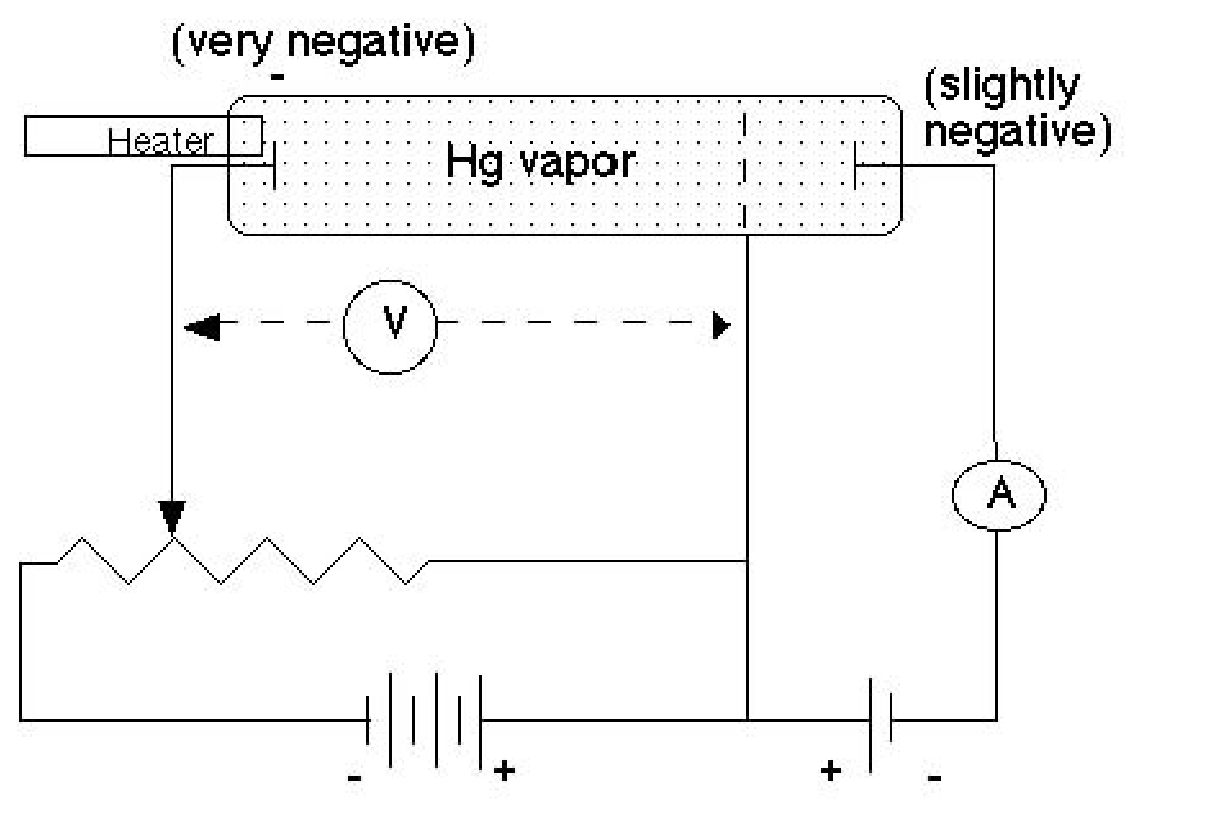
\includegraphics[clip,width=7cm]{BohrModel/4-3.ps}
\caption{夫兰克-赫兹实验示意}\label{Feank-Hertz_experiment_device}
\end{center}
\end{figure}

夫兰克-赫兹实验的装置如图\ref{Feank-Hertz_experiment_device}所示.
水银(汞,Hg)蒸汽被放在真空管内, 电子从阴极射出后, 被电势$V$加速,
然后到达阳极, 阳极是栅栏状的, 阳极后面还有一个微弱的反向电压,
反向电压比加速电压($V$)弱的多,
再后面是个集电极(类似真空三极管,发射极,基极和集电极)。

\begin{figure}[h]
\begin{center}
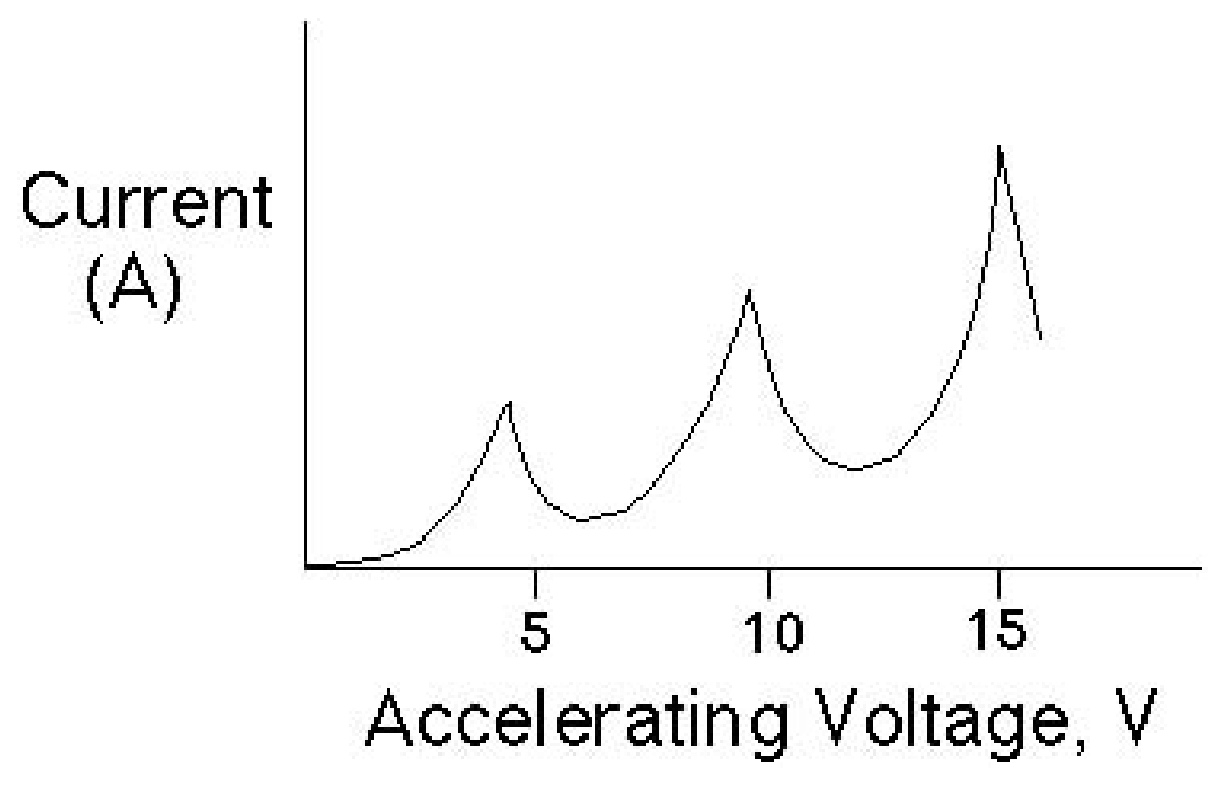
\includegraphics[clip,width=6cm]{BohrModel/4-4.ps}
\caption{夫兰克-赫兹实验:电流随电压增大以4.9V为周期,周期性地变大变小}\label{Frank-Hertz_experiment_result}
\end{center}
\end{figure}

实验测量的是加速电压($V$)和通过集电极电流($I$)之间的关系,实验结果见图\ref{Frank-Hertz_experiment_result}.
可见这里存在一个约$4.9$伏的周期,每$4.9$伏周期,集电极电流会周期性的变大,达到峰值,然后陡峭地变小。

\index{Stationary state: 定态}

这$4.9$伏的周期性可被玻尔模型所解释. 根据玻尔模型,
原子中存在一系列的定态(stationary states),
当原子由一个定态跃迁到另一定态时, 可相应地吸收或放出一个光子,
并满足频率关系(frequency relation):$h\nu =E_2 - E_1$.
$4.9$伏的周期性说明在汞原子的第一激发态与基态间能量差是$4.9eV$。

当加速电压处于$0-4.9$伏区间时, 电子将获得$0-4.9eV$的动能,
电子可能与汞原子发生弹性碰撞或非弹性碰撞,
如发生非弹性碰撞电子将损失部分能量, 而汞原子将获得部分能量.
但根据玻尔模型, 小于$4.9eV$的能量是不足以使汞原子发生跃迁的,
因此只能发生弹性散射, 电子在弹性散射的过程中并不损失能量,
因此当电子达到阳极时具有大于$0$的动能, 可以克服反向电压达到集电极,
因此表现为有电流, 并且随着加速电压的增大, 电流也相应增大.

当加速电压正好为$4.9$伏时, 电子具有$4.9eV$的动能,
可与汞原子发生非弹性散射, 汞原子被激发到激发态,
电子损失$4.9eV$后动能为0, 无法克服反向电压, 因此表现为电流急剧下跌。

当加速电压达到两倍$4.9$伏时,
则有可能发生两次电子与汞原子的非弹性散射,
因此将出现第二个峰。如果继续增大加速电压,
还可能出现更多的峰。如果电子能量大到足以把汞原子激发到更高激发态的能量,
则可以出现不是$4.9$伏周期的峰。

观察夫兰克-赫兹实验的实验曲线, 另一特征是电流波谷取值是逐渐变大的,
这可以解释为总有部分电子未发生与汞原子的非弹性散射就到达了阳极,
从而肯定会到达集电极。发生$N+1$次非弹性散射的几率要小于只发生$N$次非弹性散射的几率,
因此随着加速电压的增大会有更多的电子以非零动能到达阳极,
体现为电流波谷取值越来越高。

还可以考虑更多因素, 比如无规则热运动对夫兰克-赫兹实验曲线的影响,
将使曲线更加圆滑等等。但这些已经属于实验中不太重要的细节了。

1925年夫兰克和赫兹因夫兰克-赫兹实验共同获得诺贝尔物理学奖。


\subsubsection{X射线特征辐射}

如图~\ref{xray-spec},X射线谱由连续谱(continuous
spectrum)和特征谱(characteristic spectrum)两部分组成。
1913年,莫塞莱(Moseley)在测量了从铝到金共38种元素的光谱后发现X射线特征频率的平方根对原子序数$Z$作图,
满足线形关系:

\begin{equation}
\nu _{K_\alpha  }  = 0.248 \times 10^{16} (Z - 1)^2 Hz
\end{equation}

\index{Moseley's law: 莫塞莱定律}

\begin{figure}[h]
\begin{center}
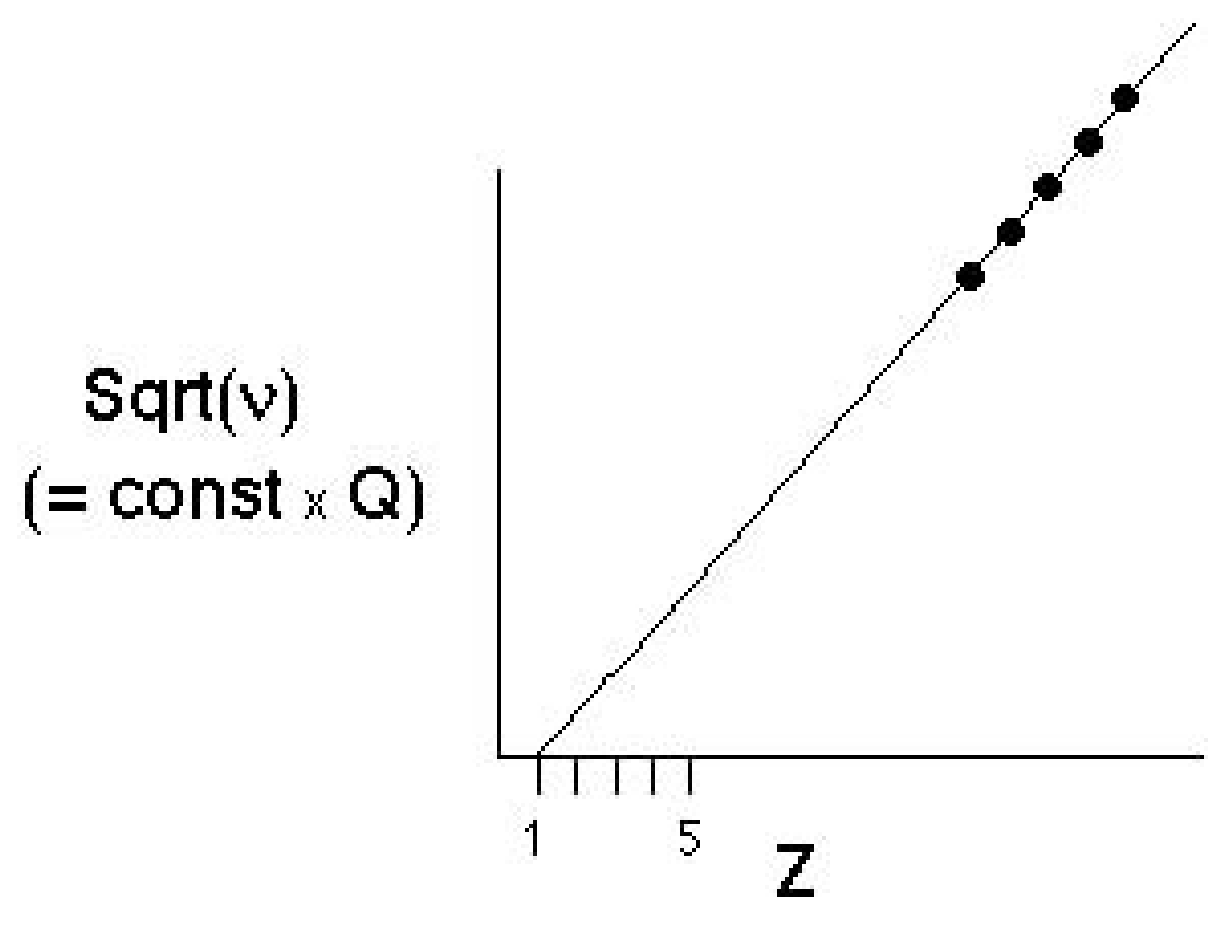
\includegraphics[clip,width=7cm]{BohrModel/4-5.ps}
\caption{X射线特征频率的平方根对原子序数Z作图满足线形关系}
\end{center}
\end{figure}

根据玻尔理论:

\begin{equation}
\nu  = cRZ^2 \left( {\frac{1}{{1^2 }} - \frac{1}{{2^2 }}} \right) \approx 0.246 \times 10^{16} Z^2 Hz
\end{equation}

公式中,$Z-1$表明跃迁电子受到$Z-1$个正电荷的有效电磁相互作用。

$K_\alpha $射线可解释为:
入射高能电子首先从原子内层$n=1$移去一个电子形成一个内层空穴,
然后外层$n=2$处电子跳到$n=1$填补空穴, 并发出射线。考虑屏蔽效应,
有效电荷应为$Z-1$ ($n=1$电子占满时, 有2个电子, 移去1个后, 还剩1个,
与原子核整体形成$Z-1$有效电荷)。同样,
我们可以解释L线系为:由外层电子跃迁至$L$($n=2$)层发出的光频率,
实验测得有效电荷为:$Z-7.5$。

\index{Characteristic radiation: 特征辐射}


\begin{figure}[h]
\begin{center}
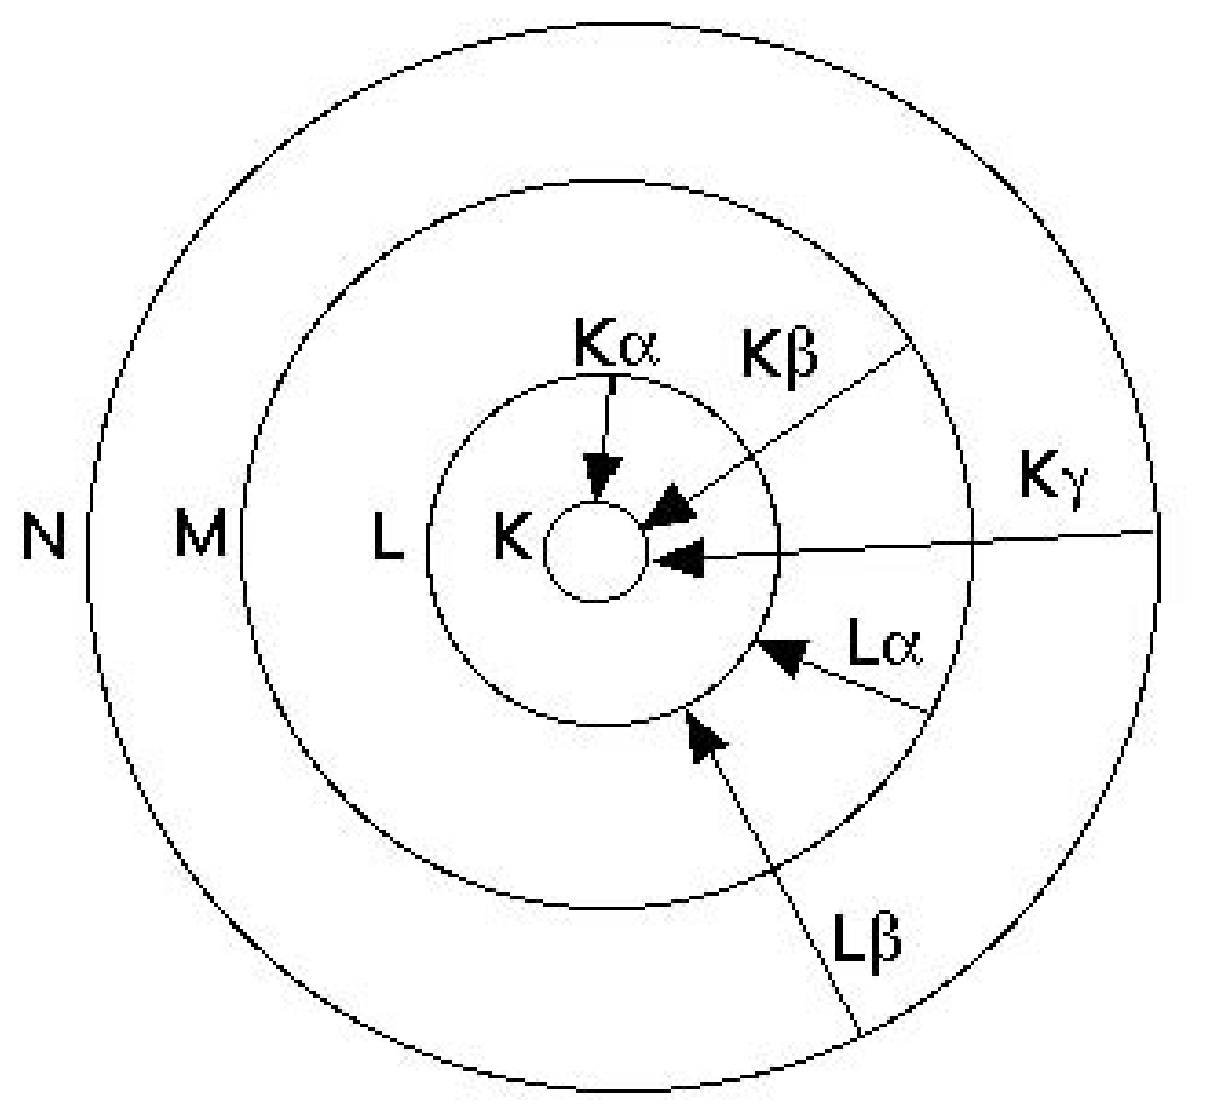
\includegraphics[clip,width=5cm]{BohrModel/4-6.ps}
\caption{X射线特征辐射:K线系(外层电子跃迁至n=1层)与L线系(外层电子跃迁至n=2层)}
\end{center}
\end{figure}



X射线的吸收限(吸收边缘):让X射线照射物体(吸收体),显然当入射X射线频率越高,吸收系数越小,
透射能力越强。但当入射X射线能量足以使一个$n=1$电子脱离原子时,则引起原子的共振吸收,对应为$K$吸收边缘。
同样也会存在$L$吸收边缘,$M$吸收边缘。如图:X射线由低频到高频分别是$L$吸收边缘和$K$吸收边缘。

\begin{figure}[h]
\begin{center}
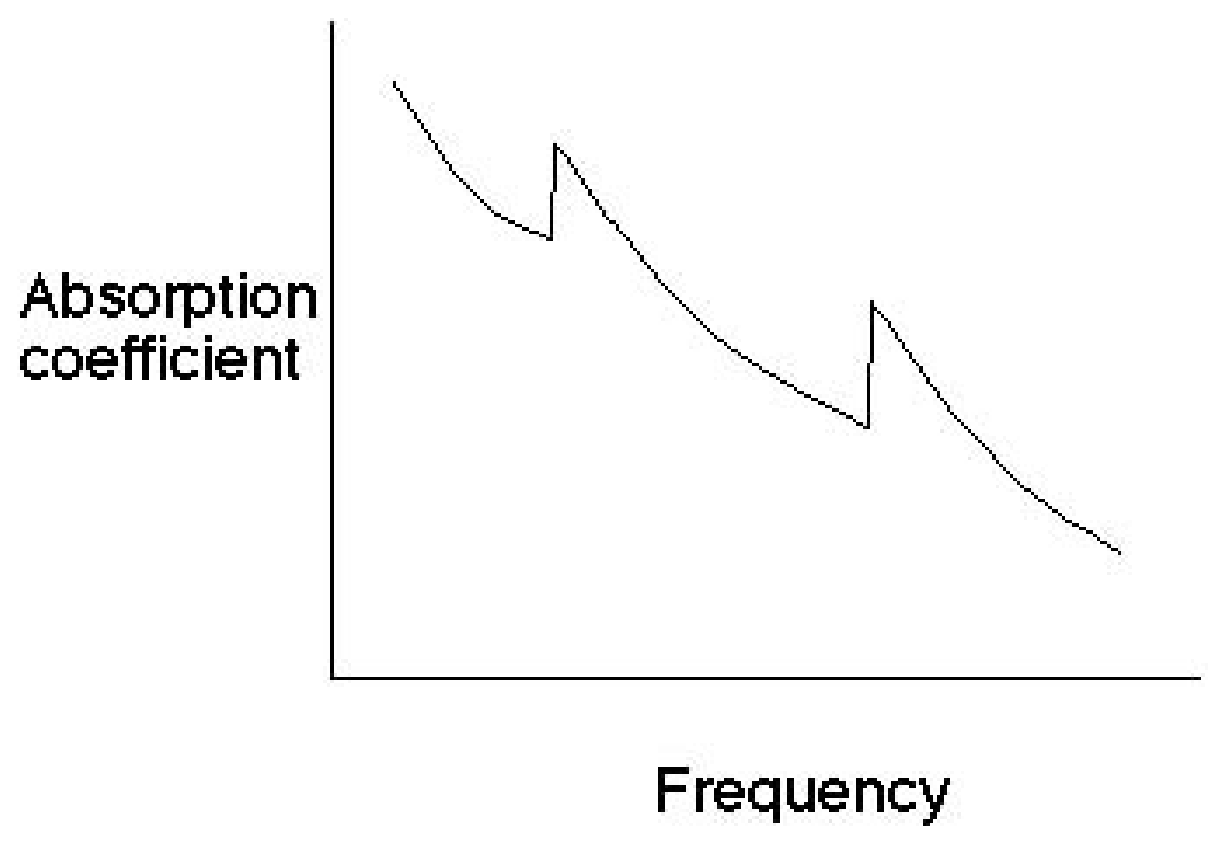
\includegraphics[clip,width=5cm]{BohrModel/4-8.ps}
\caption{X射线的吸收边缘}
\end{center}
\end{figure}

这是X射线成像技术的物理原理,如在医疗诊断中常用的CT(Computed
tomography)技术。


\subsubsection{俄歇效应}

\index{Auger effect: 俄歇效应}

\index{Auger electron: 俄歇电子}

原子壳层中产生空穴后, 产生X射线仅是释放能量的一种途径,
另一种途径是不释放X射线, 而把能量传递给另一层中的一个电子,
这个电子可以脱离原子, 称为俄歇电子,
这个过程称为俄歇电子发射。这个现象, 是法国科学家俄歇(P.
Auger)1923年发现的。一般说来, 轻元素, 发射俄歇电子的几率较大,
重元素发射X射线的几率较大。俄歇电子的动能完全决定于元素的本性,
因此对俄歇电子的测量也是进行材料分析的手段。


\begin{figure}[h]
\begin{center}
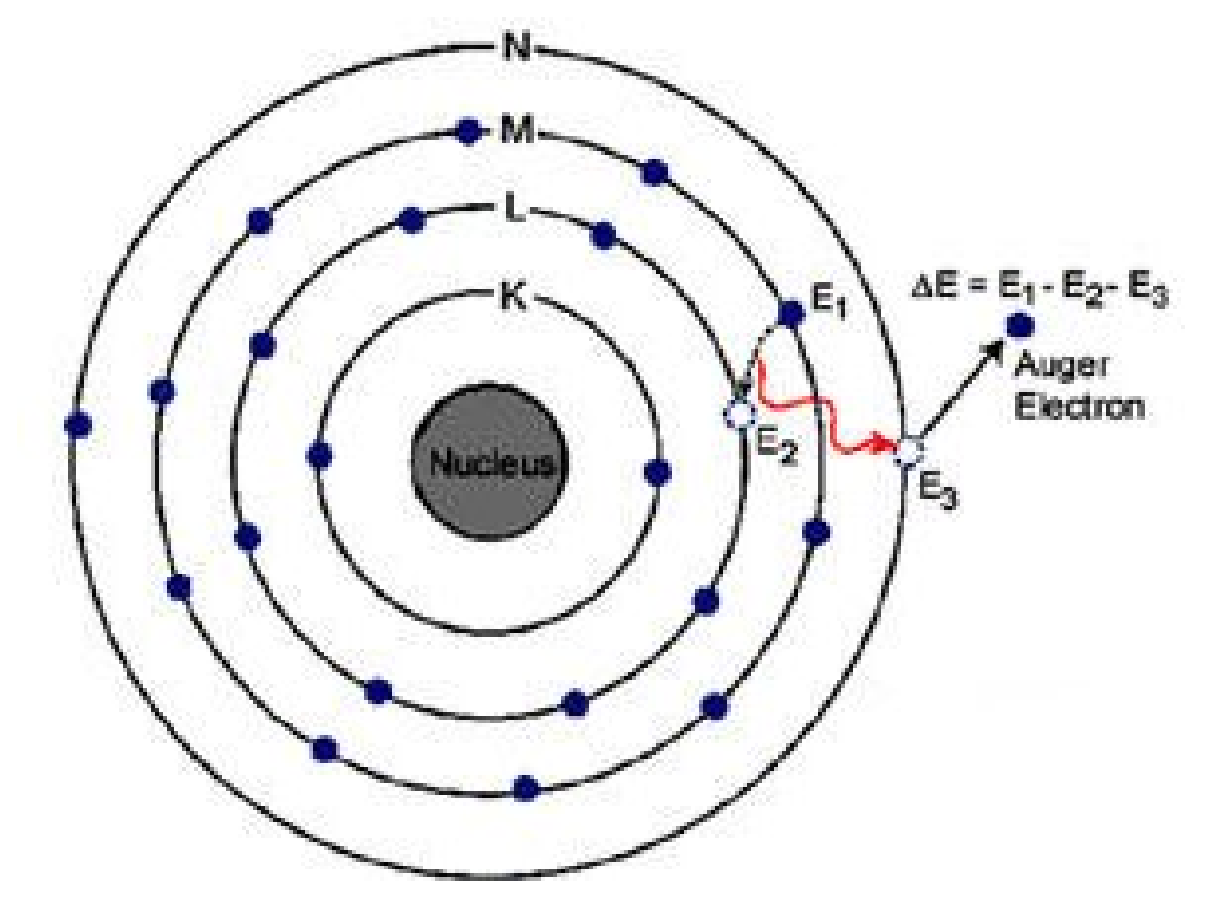
\includegraphics[clip,width=5cm]{BohrModel/auger-effect.ps}
\caption{俄歇电子发射}\label{auger electron}
\end{center}
\end{figure}


如图\ref{auger electron}, 较高能级电子湮灭空穴放出能量$E_1 - E_2$,
这个能量会激发某外层电子脱离原子而成为自由的,
在这个过程中要消耗能量$E_3$, 最终发射出的俄歇电子动能为: $E_k = E_1
- E_2 - E_3$



\subsection{玻尔-索末菲量子化条件}

\index{Bohr-Sommerfeld quantization condition:
玻尔-索末菲量子化条件}

玻尔角动量量子化条件仅适用于圆形轨道,
索末菲把玻尔量子化条件:$L = mvr = n\hbar $推广为:

\begin{equation}\label{Sommerfeld Condition}
    \oint {pdq = nh}
\end{equation}

其中$p$,$q$是一对共轭的正则坐标与正则动量,闭合回路积分代表对周期运动积分一个周期\footnote{
有兴趣的同学, 可自学: 褚圣麟编《原子物理学》, 第2.6节, pp48-55;
用这种方法可推出考虑相对论效应后的光谱项是:

\begin{equation*}
T(n,n_{\phi})=\frac{RZ^2}{n^2}+\frac{Rz^4\alpha^2}{n^4}\left(
\frac{n}{n_{\phi}}-\frac{3}{4}\right)+...,
\end{equation*}

即褚圣麟书中pp55中第(16)式。

},但有时这样作会求出很荒谬的结果。

\index{Canonical coordinate: 正则坐标}

\index{Canonical momentum: 正则动量}


\subsubsection*{卢瑟福对玻尔理论的批评}

玻尔理论在卢瑟福模型基础上, 用经典力学处理电子围绕原子核的运动,
引入了定态假设、角动量量子化条件。但这些多少带有人为的性质,
而不是严密的理论体系。卢瑟福在1913年3月20日给玻尔的信中写道\footnote{《尼耳斯·玻尔集》第二卷,
pp112}:


\begin{quote}
    你的关于氢光谱的起源方式的想法是很巧妙的, 而且看来也是很好用的;
    但是,
    普朗克概念和旧力学的混合却使人很难对什么是它的基础形成一个物理概念。在我看来,
    你的假说中有一个严重的困难,
    这个困难我毫不怀疑地认为你也充分意识到了, 那就是,
    当电子从一个定态过渡到另一个定态时,
    它怎么决定将以什么频率来振动呢? 在我看来,
    你必须假设电子事先就知道它将在什么地方停下来。
\end{quote}

\index{Old quantum theory: 旧量子论}


我们现在知道玻尔理论不是真正意义上的量子力学,
因此也称作``旧量子论''或``半经典的量子力学''。
玻尔等也尝试推广玻尔模型以适用于更复杂的一些原子(如氦),
但都失败了, 此外玻尔模型只能解释氢光谱线的位置,
而不能解释谱线的强度。因此为玻尔模型提供一个更坚实的理论基础,
发展出能够一般性地解决原子光谱现象的新力学就成为自然的任务。

\subsection*{物理常数}

\begin{itemize}
  \item 万有引力常数: $G = 6.67 \times 10^{ - 11} m^3 \cdot kg^{-1} \cdot s^{-2} $

\item 精细结构常数: $\frac{e^2}{4 \pi \epsilon_0 \hbar c} = \alpha \approx \frac{1}{137}$

  \item 氢原子的电离能: $E_{\infty} = 13.6eV$
  \item 氢原子的第一玻尔半径: $a_0 = r_1 \approx 0.053 nm$, $r_n = n^2 a_0$

  \item 氢原子的第一玻尔速度: $v_1 = \alpha c$, $v_n = \frac{\alpha c}{n}$
\end{itemize}


\subsection*{练习}


\begin{enumerate}
\item 假设恒星可按绝对黑体处理, 估算恒星表面温度为多少时, 恒星发出的辐射可使其周围的氢电离。

解: 氢原子的电离能是$13.6eV$, 相当于: $13.6 \times 1.602 \times
10^{-19} = 2.18 \times 10^{-18} J$, 能使氢原子电离的光子的波长是,

\begin{equation*}
\lambda = \frac{hc}{\varepsilon}=\frac{6.626 \times 10^{-34} \times
3.0 \times 10^8}{2.18 \times 10^{-18}} = 9.1 \times 10^{-8}m
\end{equation*}

根据维恩位移定律, $\lambda_{max} T = 2.898 \times 10^{-3} m \cdot
K$,

\begin{equation*}
T = \frac{2.898 \times 10^{-3}}{9.1 \times 10^{-8}}=3.0\times 10^4 K
\end{equation*}

即需要大约三万K使恒星附近的氢原子电离.
或者说当整个宇宙的背景温度是三万K时, 自由的氢原子是不可能存在的,
只有质子和电子.

作为比较, 我们知道像太阳那样的恒星, 其表面温度是大约5780K.
对应$\lambda_{max}$是:

\begin{equation*}
\lambda_{max} = \frac{2.898 \times 10^{-3}}{5780} = 500 nm
\end{equation*}

能量是:

\begin{equation*}
\varepsilon =h \nu = \frac{hc}{\lambda}= \frac{6.626 \times 10^{-34}
\times 3.0 \times 10^8}{5.0 \times 10^{-7}}= 4.0 \times 10^{-19} J
\end{equation*}

相当于: $\frac{4.0 \times 10^{-19}}{1.602 \times 10^{-19}}=2.5
\text{eV}$.

如果是一颗红星, 取$\lambda_{max}=650 nm =6.5 \times 10^{-7}m$,
红星表面的温度是:

\begin{equation*}
T = \frac{2.898 \times 10^{-3}}{6.5 \times 10^{-7}}=4400K
\end{equation*}

即红星表面温度仍高达4400K.

  \item 电子偶素是由一个正电子和一个电子所组成的一种束缚系统,试求:
(1)基态时两电子之间的距离;(2)基态电子的电离能和由基态到第一激发态的激发能;
(3)由第一激发态退激到基态所放光子的波长。

\item 电子和质子间的引力是$\frac{Gm_pm_e}{r^2}$, 假设只考虑引力而忽略电磁相互作用. 按照玻尔理论估算氢原子的第一玻尔半径(请把最终结果用光年表示).

\item $He^+$离子的电离能是多少? (答: $13.6 eV \times 4 = 54.4 eV$)

\item 利用“玻尔-索末菲量子化条件”求一维谐振子的能量,并说明其是量子化的。

\end{enumerate}


\subsection*{阅读}

关于里德堡原子和量子信息(量子计算),请阅读:

Quantum information with Rydberg atoms, Rev. Mod. Phys. 82,
2313–2363 (2010).

\url{http://rmp.aps.org/abstract/RMP/v82/i3/p2313_1}